\chapter{Monte Carlo Models of Signal and Background} \label{ch:monte_carlo}

\section{Signal modeling}\label{sec:signal_modeling}

Simulated gluino pair-production events are generated for use in the analysis.
Separate samples are generated for the direct decay and cascade decay models described in~\ref{subsec:rpv_gluino}.
For the direct decay model, events are generated for gluino mass ranging from $900~GeV$ to $1.8~TeV$ .
For the cascade model, the gluino mass is varied from $750~GeV$ up to $2.1~TeV$, with the neutralino mass ranging from $450~GeV$ to $1.9~TeV$ .
For all signal points, the neutralino mass is lower than the gluino mass, as is required by the decay modes of interest.
Signal events are simulated for a discrete set of mass points.
Figure~\ref{fig:signal_cascade_grid} indicates the $\left(m_{\tilde{g}}, m_{\tilde{\chi}_1^0}\right)$ points for which signal evens were generated.
This grid of signal points is chosen to cover the range of masses that the analysis is expected to be sensitive to.
The grid points are spaced closer together in the high-$m_{\tilde{g}}$ region, near where the expected limits (\ref{subsec:results_limits}) lie.

\begin{figure}[!ht]
    \centering

    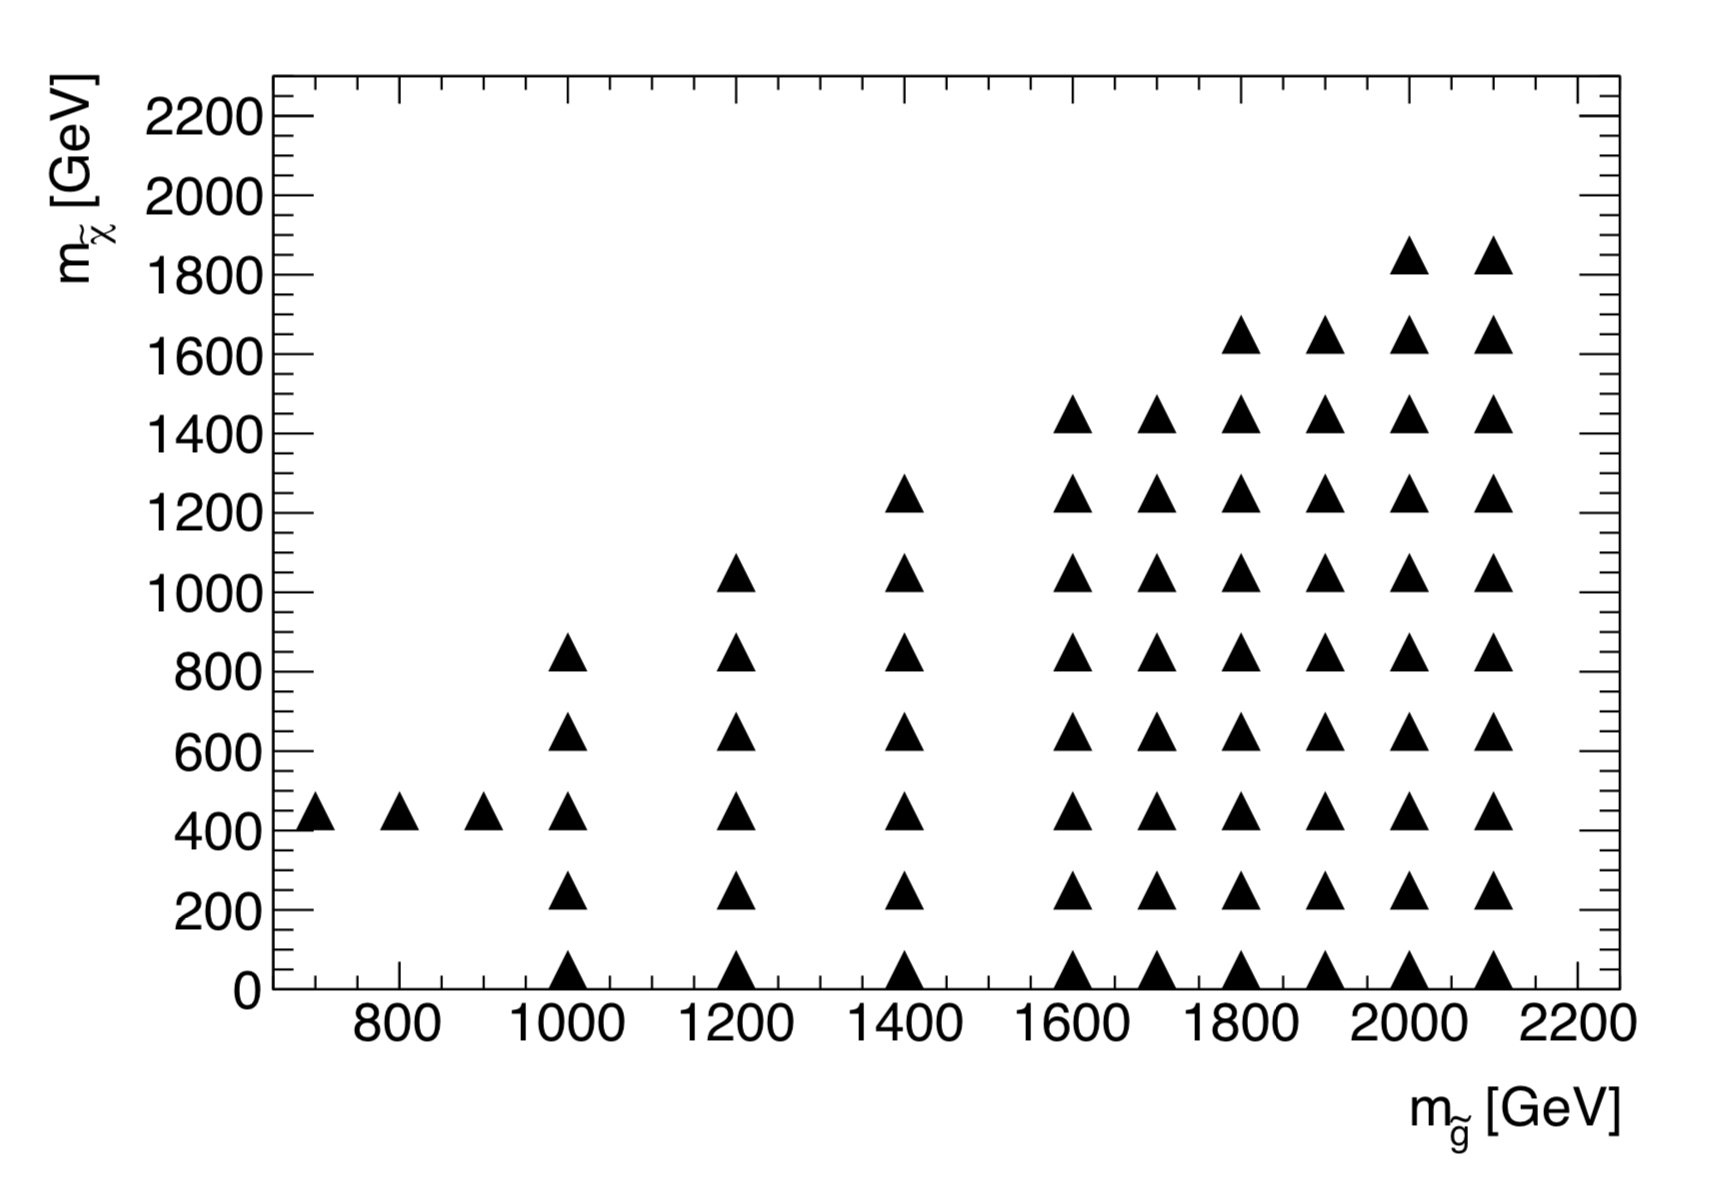
\includegraphics[width=0.9\linewidth]{signal_cascade_grid}

    \caption{The grid of gluino and neutralino masses for which simulated cascade decay events were generated.
    The triangles indicate the mass points for which simulated events were generated.}

    \label{fig:signal_cascade_grid}
\end{figure}

\subsection{Event generation}\label{subsec:signal_event_gen}

Matrix elements for gluino pair production are generated with \textsc{MadGraph\_aMC@NLO} v2.3.3, which is a convenient framework for calculating arbitrary matrix elements at up to next-to-leading order (NLO)~\cite{signal-madgraph}.
\textsc{MadGraph} allows the user to specify the theory being used and values for the free parameters, then it constructs and calculates the necessary Feynman diagrams.
In this analysis, matrix elements are calculated at leading order (LO).
In the pair-production matrix elements, up two two additional partons are allowed to be produced along with the gluino pair.

To model the parts of the collision environment described in section~\ref{sec:jet_collisions}, such as the underlying event, parton shower, and fragmentation, \textsc{Pythia} 8.186 is used~\cite{signal-pythia}.
Interfacing \textsc{MadGraph} and \textsc{Pythia} is made possible by a standardized file format known as Les Houches Event Format (LHEF)~\cite{signal-lhef}.

As discussed in section~\ref{sec:jet_collisions}, there are non-perturbative processes that occur in proton-proton collisions, which cannot be directly calculated from first principles.
This processes can be parameterized and approximated in a program like \textsc{Pythia}, requiring many free parameters with values that must be constrained using data.
The process of inferring these parameters so that the calculations match the data is known as tuning.
For this analysis the A14 set of tuned parameter values are used to model the underlying event in \textsc{Pythia}~\cite{signal-pythia-a14,signal-pythia-tunes}.
The parton distribution functions (PDFs) used for the simulated signal generation are from the NNPDF2.3LO set~\cite{signal-nnpdf}.

\subsection{Cross-section}\label{subsec:signal_cross_section}
In order to estimate the expected signal yield and uncertainty, the nominal production cross section and its uncertainty must be known.
Gluino pair-production cross-sections have been calculated at a range of center-of-mass energies, and the results are summarized in~\cite{signal-xsec}.
The gluino pair-production cross-section and its uncertainty over a range of gluino masses can be seen in~\ref{fig:signal_xsec}.

\begin{figure}[!ht]\centering
    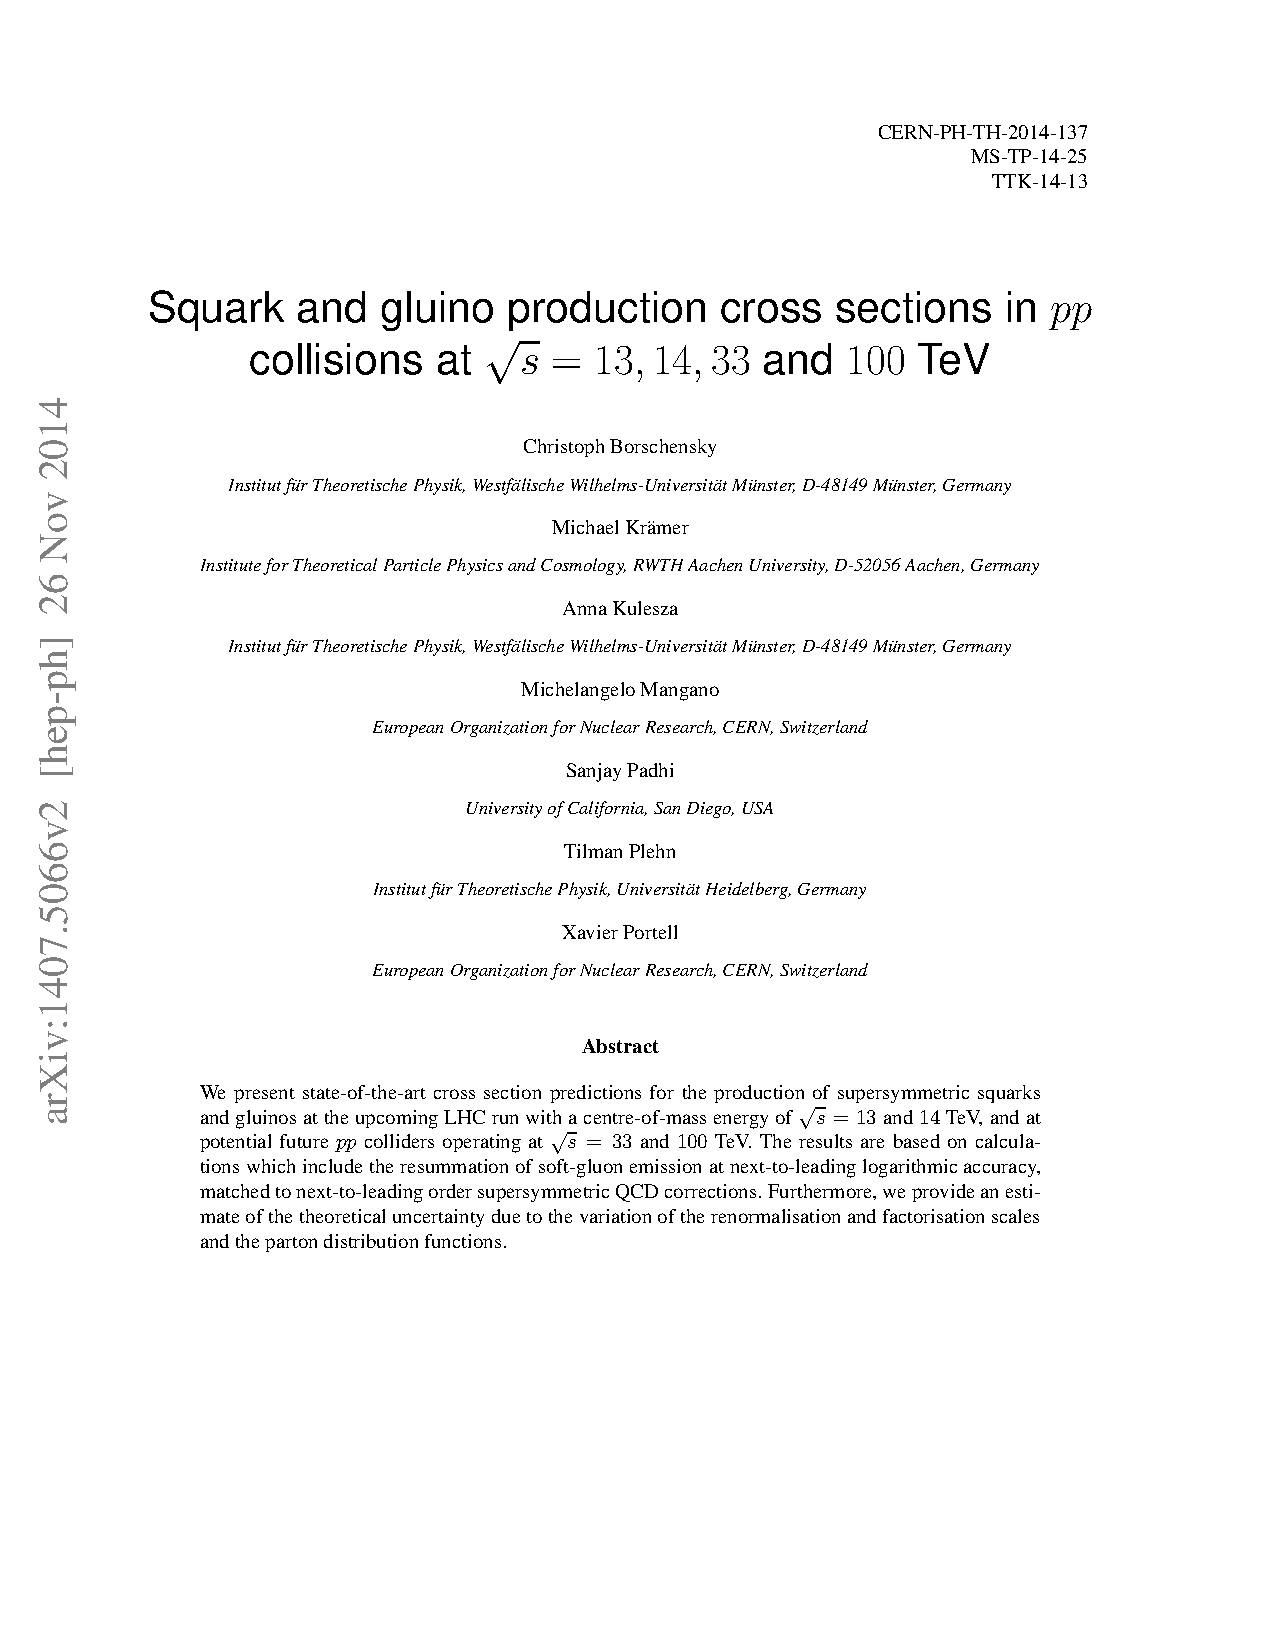
\includegraphics[width=0.9\linewidth]{signal_xsec}
    \caption{Gluino pair-production cross-section and uncertainty for $\sqrt{13}~TeV$ proton-proton collisions at the LHC, calculated at NLO+NLL~\cite{signal-xsec}.}
    \label{fig:signal_xsec}
\end{figure}

\subsection{Fast simulation with Atlfast-II}\label{subsec:fastsim}

Simulation of the detector response to physics events requires large amounts of computational resources.
In order to reduce the cost of generating large samples of simulated events, a faster version of the detector response simulation, called Atlfast-II has been developed~\cite{mc-atlfast}.
Fast simulation with Atlfast-II (AFII) can greatly reduce the time required to generate these simulated events, but makes several simplifications that can lead to less precise results.

A comparison between the full detector simulation (FullSim) and AFII was performed to find out if using AFII would reduce the sensitivity of the search or otherwise affect the analysis.
Very good agreement between FullSim and AFII-simulated events is observed across a range of kinematic observables relevant to this analysis.
As a result, AFII simulation is used for generating signal events for all of the grid points used in the limit-setting.
Full simulation events are also generated for a few representative signal points.

For the FullSim/AFII comparison, full simulation events for the decay modes described in chapter~\ref{ch:analysis_overview} were not available, but a very similar signal was used.
In this case, pair-produced gluinos each decay to a neutralino + $t\bar{t}$, and the neutralinos each decay through a $\lambda''$ vertex to three light quarks.
This process is illustrated in~\ref{fig:mc_gtt}.
The benchmark model used in this study has $m_{\tilde{g}}=1250~GeV$ and $m_{\tilde{\chi}}=450~GeV$.
Events used in this study are required to have $H_{T}>1~TeV$ and lead jet $p_{T}>200~GeV$.
Large-$R$ jets are fully calibrated using FullSim calibration and required to have $p_{T}$ of at least $100~GeV$ and $|\eta|$ less than $2.8$.
Jet mass response is defined as $m_{reco}/m_{truth}$, where $m_{reco}$ is the reconstructed jet mass and $m_{truth}$ is the mass of jets clustered from truth particles.

Figure~\ref{fig:afii_mass_response} shows the large-$R$ jet mass response vs. truth mass and vs. truth $p_{T}$ for large-$R$ jets with $p_{T}>100~GeV$ and $|\eta|<2.8$.
The points and error bars show the best-fit mean and width for a Gaussian fit to the core of the distribution in each bin.
Figure~\ref{fig:afii_kinematics} shows the distribution of large-$R$ jet kinematic observables $m$, $\eta$, $\phi$, and $p_{T}$ for both FullSim and AFII, along with the ratio of each bin in the bottom panel of each plot.
Figure~\ref{fig:afii_mj} shows the large-$R$ jet multiplicity histogram for reconstructed jets using both AFII and FullSim, and the distributions of $M_{J}^{\Sigma}$ for events with at least 5 large-$R$ jets.
In all cases, very good agreement is observed between FullSim and AFII distributions.

\begin{figure}[!ht]\centering
    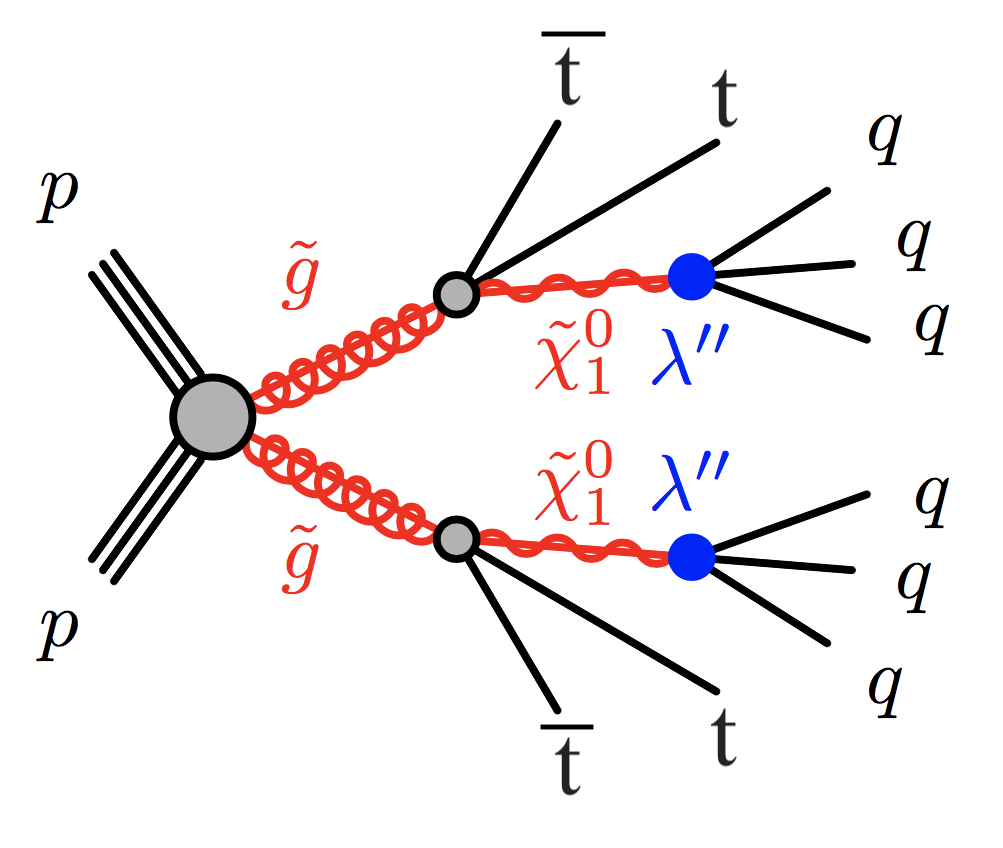
\includegraphics[width=0.6\linewidth]{mc_gtt}
    \caption{The process used for the AFII/FullSim comparison study.
    The signal is very similar to the cascade decay model used in the search, but the gluinos decay to a neutralino+$t\bar{t}$ rather than a neutralino and two light quarks.}
    \label{fig:mc_gtt}
\end{figure}

\begin{figure}[!ht]\centering
    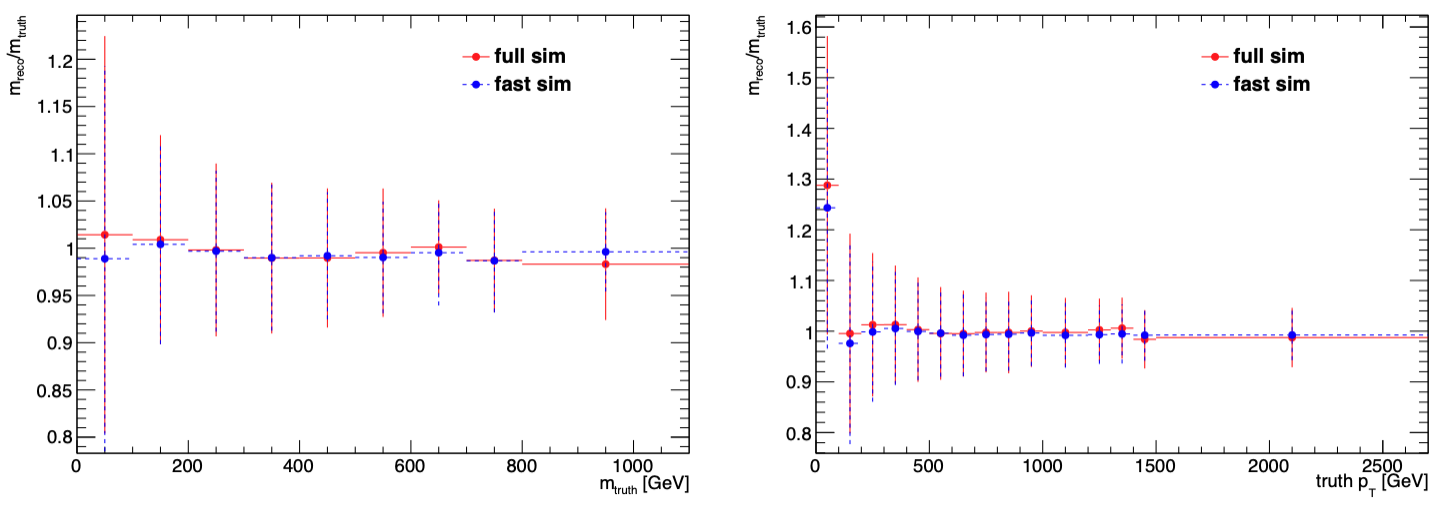
\includegraphics[width=0.9\linewidth]{mc_afII_mass_response}
    \caption{Jet mass response vs true jet mass (left) and truth jet $p_{T}$ for simulated signal events using both the full detector simulation (full sim) and Atlfast-II (fast sim).
    Points and error bars show the best-fit mean and width for a Gaussian fit to the core of the distribution in each bin.
    The model used for this study is similar to the cascade decay model described in~\ref{ch:analysis_overview}, except each gluino decays to a neutralino + $t\bar{t}$ rather than a neutralino and two light quarks.
    The gluino mass is $1250~GeV$ and neutralino mass is $450~GeV$.
    Jets are required to have $p_{T}$ greater than $100~GeV$ and $|\eta|<2.8$.
    }
    \label{fig:afii_mass_response}
\end{figure}

\begin{figure}[!ht]\centering
    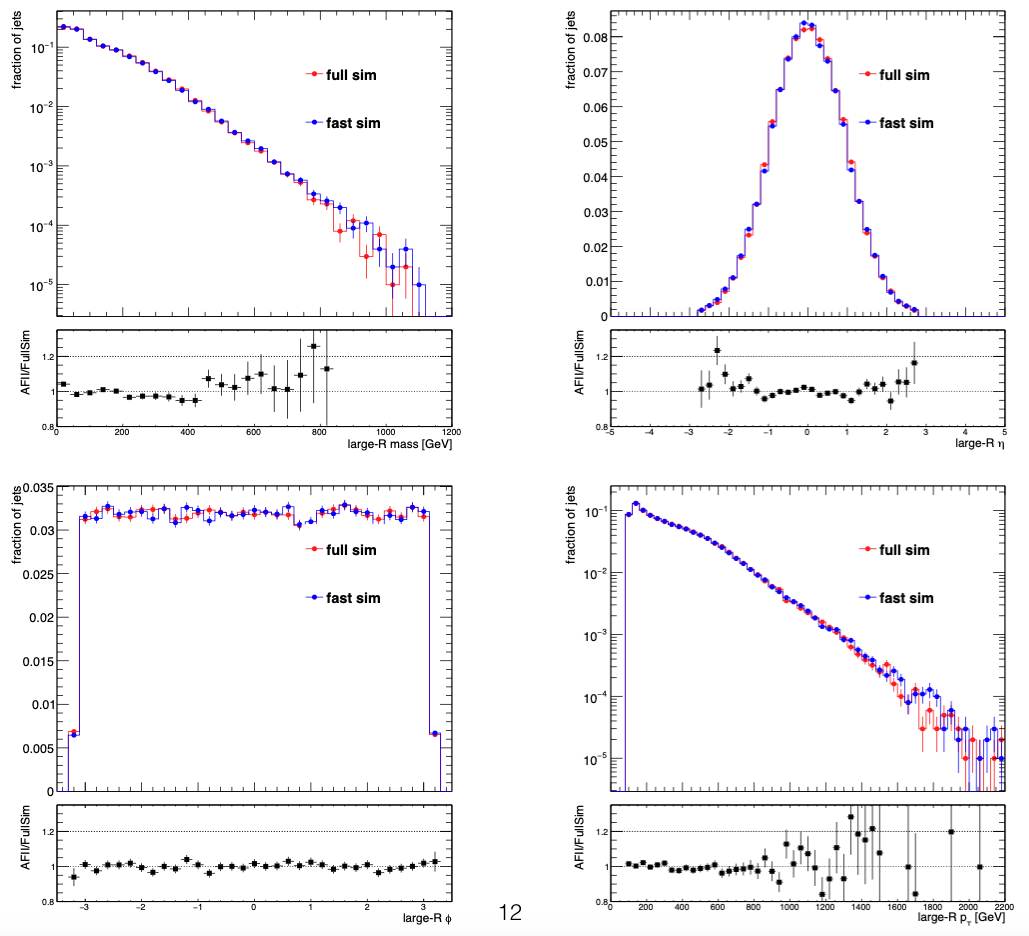
\includegraphics[width=0.9\linewidth]{mc_afii_kinematics}
    \caption{Kinematic distributions of large-$R$ jets for simulated events using both the full detector simulation (full sim) and Atlfast-II (fast sim).
    The model used for this study is similar to the cascade decay model described in~\ref{ch:analysis_overview}, except each gluino decays to a neutralino + $t\bar{t}$ rather than a neutralino and two light quarks.
    The gluino mass is $1250~GeV$ and neutralino mass is $450~GeV$.
    Jets are required to have $p_{T}$ greater than $100~GeV$ and $|\eta|<2.8$.
    }
    \label{fig:afii_kinematics}
\end{figure}

\begin{figure}[!ht]\centering
    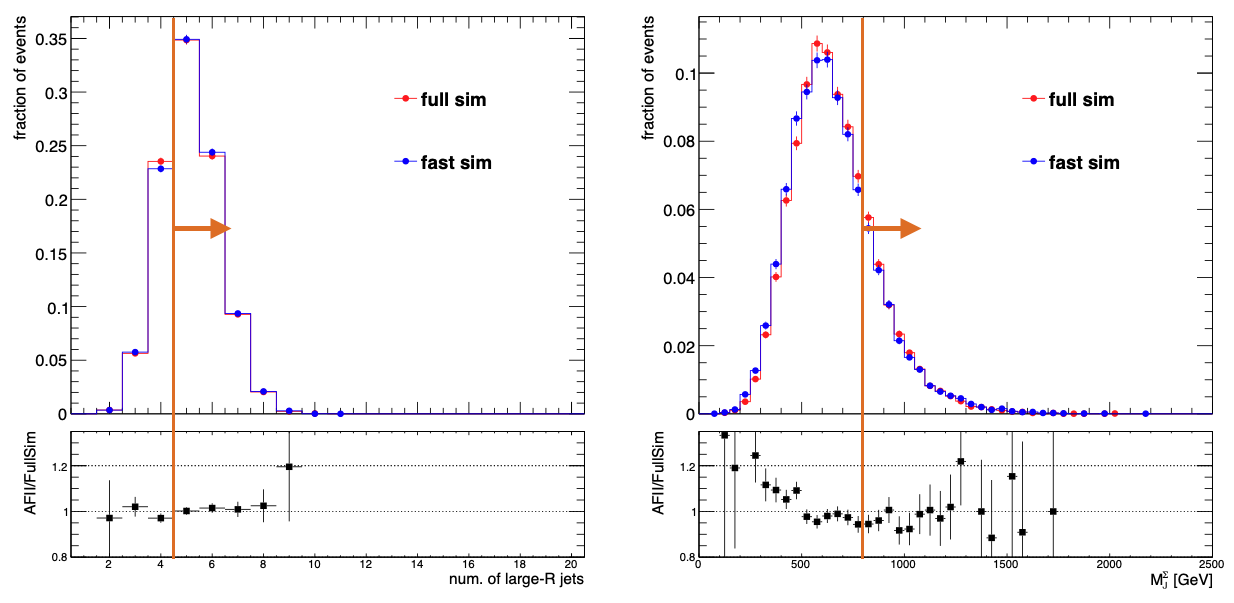
\includegraphics[width=0.9\linewidth]{mc_afii_mj}
    \caption{Jet multiplicity and distribution (left) and $M_{J}^{\Sigma}$ for events with at least 5 large-$R$ jets (right) for simulated events using both the full detector simulation (full sim) and Atlfast-II (fast sim).
    The model used for this study is similar to the cascade decay model described in~\ref{ch:analysis_overview}, except each gluino decays to a neutralino + $t\bar{t}$ rather than a neutralino and two light quarks.
    The gluino mass is $1250~GeV$ and neutralino mass is $450~GeV$.
    Jets are required to have $p_{T}$ greater than $100~GeV$ and $|\eta|<2.8$.}
    \label{fig:afii_mj}
\end{figure}

\section{Background modeling}\label{sec:bkg_modeling}

Background estimation for this analysis is done with a fully data-driven method that does not rely on Monte Carlo to make predictions.
However, simulated background events are generated and studied in order to test and validate the data-driven background estimation method.
This process is detailed in~\ref{sec:bkg_monte_carlo}.

The Pythia8 multijet background sample is generated using Pythia8 8.186~\cite{signal-pythia}.
Like with the signal samples described in~\ref{subsec:signal_event_gen}, the A14 underlying-event tune~\cite{signal-pythia,signal-pythia-a14} and the NNPDF2.3LO PDF sets are used~\cite{signal-nnpdf}.
Multijet samples are also generated with Sherpa and Herwig++.
The $t\bar{t}$ events are generated with Powheg-Box v2~\cite{mc-powheg} with the CT10 PDF set~\cite{mc-ct10-pdf}.

The differential multijet cross section falls drastically with increasing $p_{T}$, so multijet events are not generated with a probability distribution proportional to the differential cross section.
If they were, the result would be enormous numbers of events with only low-$p_{T}$ jets, and very few events with high-$p_{T}$, resulting in very large statistical uncertainties for the high-$p_{T}$ jet events.
Instead, multijet events are generated in slices, where each slice has a minimum requirement on the leading-jet $p_{T}$.
Approximately equal numbers of events can then be generated for each slice, and re-weighted according to the relative cross-section of each slice.
Using this method, the statistical uncertainty is more constant across a wide range of jet $p_{T}$.
The lowest-$p_{T}$ slice that passes the event selection for this analysis has a lead-jet range of $160~GeV - 400~GeV$.
For this slice, just under 16 million simulated events are generated, which corresponds to an effective luminosity of $1.9~fb^{-1}$.